%; whizzy document
% latex beamer presentation.
% platex, latex-beamer でコンパイルすることを想定。 


%     Tokyo Debian Meeting resources
%     Copyright (C) 2006 Junichi Uekawa

%     This program is free software; you can redistribute it and/or modify
%     it under the terms of the GNU General Public License as published by
%     the Free Software Foundation; either version 2 of the License, or
%     (at your option) any later version.

%     This program is distributed in the hope that it will be useful,
%     but WITHOUT ANY WARRANTY; without even the implied warranty of
%     MERCHANTABILITY or FITNESS FOR A PARTICULAR PURPOSE.  See the
%     GNU General Public License for more details.

%     You should have received a copy of the GNU General Public License
%     along with this program; if not, write to the Free Software
%     Foundation, Inc., 51 Franklin St, Fifth Floor, Boston, MA  02110-1301 USA


\documentclass[cjk,dvipdfmx]{beamer}
\usetheme{Warsaw}
%  preview (shell-command (concat "xpdf " (replace-regexp-in-string "tex$" "pdf"(buffer-file-name)) "&"))
%  presentation (shell-command (concat "xpdf -fullscreen " (replace-regexp-in-string "tex$" "pdf"(buffer-file-name)) "&"))

%http://www.naney.org/diki/dk/hyperref.html
%日本語EUC系環境の時
\AtBeginDvi{\special{pdf:tounicode EUC-UCS2}}
%シフトJIS系環境の時
%\AtBeginDvi{\special{pdf:tounicode 90ms-RKSJ-UCS2}}


\title[Debian 勉強会]{Debian勉強会}
\subtitle{2006年4月15日版}
\author{上川}
\date{2006年4月15日}

\begin{document}
\frame{\titlepage{}}

\section{進め方}
\begin{frame}
 \frametitle{本日のagenda}
\begin{itemize}
 \item 注意事項
       \begin{itemize}
	\item 飲食禁止
	\item 政治/宗教/営利活動禁止
       \end{itemize}
 \item 18:00-18:10 Social Contract 唱和
 \item 18:10-18:45 クイズ
 \item 18:55-19:30 Debian TeX
 \item 19:45-20:20 Debian Policy: source 編
 \item 20:30-20:50 前回の勉強会報告
 \item 21:00- 宴会 @ 一汁一菜 遇
\end{itemize}

\end{frame}

\section{Debianでの文書処理についてのユーザの声}

\begin{frame}
 \frametitle{ユーザの声}
... 日記や、思いつきのメモを書くためには hiki と Web ブラウザを
使っています。どこからでも更新・参照でき、最低限の文書構造を表現
できるので Wiki を使っています。難点は、hiki の編集モードが
W-ZERO3 + Opera 環境からだととても使いづらいところです。
\end{frame}

\begin{frame}
 \frametitle{ユーザの声}
基本的に議事録とかは後々メールに貼付けたり添付したりするので、bluebirdでテキ
スト作成して、他のユーザーを巻き込むような案件での文章はOpen officeを使って
相手がmicrosoft officeを使って開けるように気をつけています。相手がpowerpoint
で開くとかならずレイアウトが崩れている!と嫌みめいたメールが来ますがそこはあ
んまり気にしないようにしてます。後はよくする事がthunderbirdでメール新規作成
をしてドラフトで保存してます。検索が簡単なのとメールでのやり取りが多い&新し
くbluebirdを立ち上げなくていいので、結構便利だと思っています。
\end{frame}

\begin{frame}
 \frametitle{ユーザの声}
文書は、mailが一番おおく、つぎはtDiaryへのpublishingです。その次は
発表資料作成に、OpenOffice.orgのImpressでプレゼン資料を作ります。
長文の論文などは、p\LaTeX を使います。最終出力形態は、プラットホーム
を意識する場合が少ないpdfにすることが多いです。
英語の文書を作成するときには、辞書とスペルチェッカーが重要です。
ebviewやlookup.el、ならびにflyspell-modeはよく使います。
\end{frame}

\begin{frame}
 \frametitle{ユーザの声}
いままで Linux でドキュメントを書くことはありませんでした。プレゼンテーションの
ときは ooimpress でした。しかし、Debian 勉強会に参加して、自分でも発表を行うよう
になってから、\TeX{} に目覚め、今では会社のドキュメントも \TeX{} で書く
ようになってしま
いました。\underline{これからは Word なんかを使わず、茨の道を進んでいこうと思います。}
\end{frame}

\begin{frame}
 \frametitle{ユーザの声}
 \begin{center}
  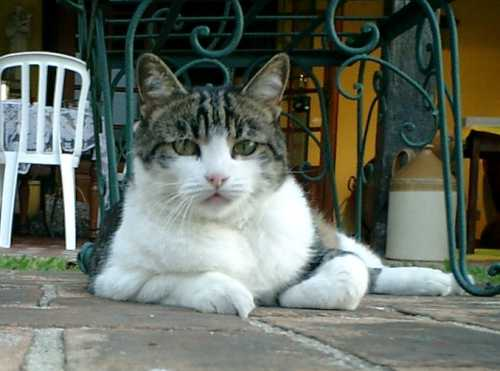
\includegraphics[height=8cm]{image200604/cat.png}
 \end{center}
\end{frame}


\section{Debian-tex policy 概説}

\begin{frame}
 \frametitle{ポリシーの存在}

\begin{center}
 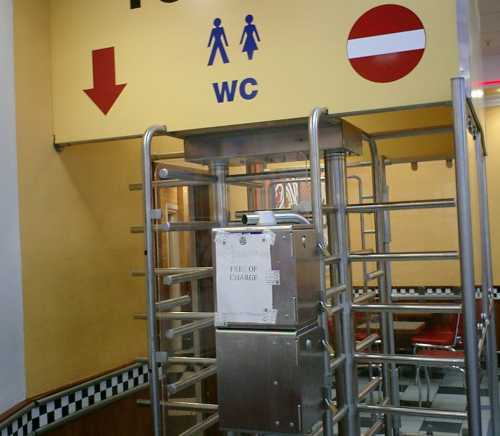
\includegraphics[height=8cm]{image200604/toilet.png}
\end{center}
\end{frame}

\begin{frame}
 \frametitle{ディレクトリツリー}
\begin{itemize}
 \item /usr/share/texmf-tetex/:  TEXMFDIST
 \item /usr/share/texmf-texlive/: TEXMFDIST
 \item /usr/share/texmf/: TEXMFMAIN
 \item /var/lib/texmf/: TEXMFSYSVAR
 \item /etc/texmf/:  TEXMFSYSCONFIG
 \item /usr/share/texmf-site/: TEXMFSITE
 \item /usr/local/share/texmf/:  TEXMFLOCAL
 \item texmf.cnf に指定してある  TEXMFHOME の値、もしくは環境変数として
       の値。
 \item 必須ではない: 各ユーザ用の設定ファイルディレクトリ TEXMFCONFIG, 生成されたファ
       イルのディレクトリ TEXMFVAR
\end{itemize}
下が最も優先される
\end{frame}

\begin{frame}
\frametitle{TeXをビルドに活用する場合}

設定ファイルを変更しないとビルドできない場合、設定ファイルのデフォルトを
変更するようにメンテナにかけあうことが推奨

\end{frame}

\section{Debian TeX 現状}

\begin{frame}
\frametitle{日本語処理}

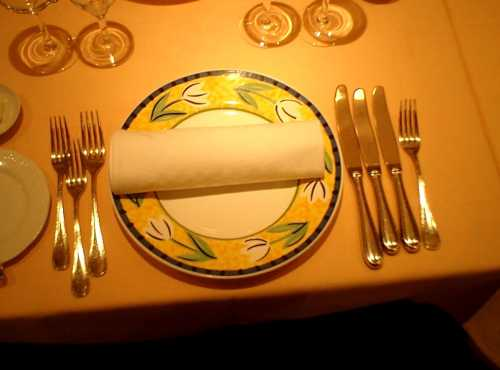
\includegraphics[width=10cm]{image200604/appetite.png}

\end{frame}

\begin{frame}
\frametitle{日本語処理}

日本語の\LaTeX 文書を処理する方法は複数存在している。
Debianに入っているパッケージが実際に使用に耐える状態なのか、調査してみた。

\LaTeX のソースファイルから PDF を生成する処理がどうなっているのかを確認
してみた。

\end{frame}

\begin{frame}
\frametitle{platexの入力文字コード}
\begin{center}
 \begin{tabular}{|c|c|}
 文字コード & 可否 \\
 \hline
 EUC-JP & ○ \\
 SJIS & × \\
 ISO-2022-JP & ○ \\
 UTF-8 & × \\
 \end{tabular}
\end{center}

\end{frame}

\begin{frame}
\frametitle{platex の PDF化}
\begin{itemize}
 \item dvipdfmx: OK
 \item dvips 経由 ps2pdf: dvips処理中にフォントが見付からない旨のエラー。
       PDFは生成されるが、日本語の文字は表示されず
 \item dvi2ps 経由 ps2pdf: gsの処理中にエラーが表示されて停止(回避可能)。
 \item pdfe\LaTeX: 直接PDFを生成できる版は存在しない
\end{itemize}
デフォルトでPDFまで生成できる状態になっているパッケージはdvipdfmxのみ。
\end{frame}

\begin{frame}
\frametitle{jlatex, multex}
小さなサンプルはコンパイル可能。

Debian勉強会資料になるとクラスファイルなどが足りずエラー。

\begin{itemize}
 \item jsarticleが無い
 \item url.styがエラーになる
\end{itemize}

p\LaTeX{}から簡単に乗り換えられる状態ではないようだ。

multexはインストールしたそのままではフォントが一部足りない。

\end{frame}

\begin{frame}
 \frametitle{cjk-latex}
インストールした状態では、サンプルがコンパイルできない。

latex-cjkパッケージとしてリニューアル作業中らしい。
\end{frame}

\begin{frame}
 \frametitle{lambda/lamed}
\begin{itemize}
 \item ``omega ($\Omega$)'' ``aleph ($\aleph$)'' : \TeX{}をUTF-8に対応させた版、それぞれの
       \LaTeX{}。
       理想としては各国語処理がこの\TeX{}で統合できる
 \item  それっぽく処理はしてくれるようなのだが、utf-8に対応できているdvi関連の
       ツールの使い方についての情報が少ないのか、そもそも存在していない
       のかはわからないが、現状、出力を表示、処理する方法がわからない。
 \item pdfe\LaTeX 版が存在しないので、日本語文書のみを処理するのであれば 
       p\LaTeX から移行してもメリットが少ない
\end{itemize}
\end{frame}

\begin{frame}
 \frametitle{先は長い}

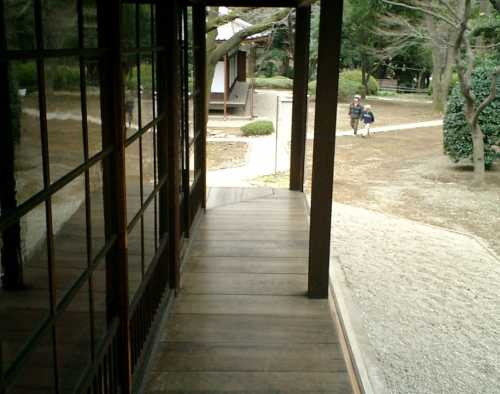
\includegraphics[width=10cm]{image200604/endscene.png}

\end{frame}

\end{document}
